\documentclass[a4paper,10pt]{article}
\usepackage[utf8]{inputenc}
\usepackage[T1]{fontenc}
\usepackage[french]{babel}
\usepackage{lmodern} %pack de police
\usepackage{tikz}

\author{Meryll \bsc{Essig}\\ Tamara \bsc{Rocacher}}
\date{\today}
\title{Complément au Cahier des Charges}


\begin{document}

\vfill
\maketitle
\vfill
\renewcommand{\abstractname}{Introduction}
\begin{abstract}
Dans le cadre de l'UE modélisation et programmation par objets 2, nous avons réalisé un projet, préalablement définit par un Cahier des Charges donné à titre de consigne.\\
Ce projet consiste en l'implémentation d'une application permettant de gérer les tâches à réaliser d'un utilisateur, sous forme de Todo List.\\
Ainsi, ce document établit les choix effectués lors de la réalisation de notre projet, dans le but de respecter au mieux les fonctionalités attendues tout en simplifiant à la fois l'implémentation et l'utilisation.
\end{abstract}
\vfill
\newpage
\renewcommand{\contentsname}{Sommaire}
\tableofcontents

\newpage
%\vfill

\section{Conception}
\subsection{Vue}
La phase de conception a permis, d'une part, de définir totalement la partie Vue.
Pour cela, nous avons choisi de n'établir qu'une seule fenêtre permettant à la fois l'affichage des tâches a réaliser sous forme de liste (1-liste), et l'affichage des champs a remplir pour créer ou modifier une tâche (2-tâche).
Ce choix repose sur le besoin de faciliter la prise en main de l'application pour l'utilisateur.
\\
De même, pour le changement du mode d'affichage de la liste de tâches (simple ou détaillé), nous avons choisi de ne pas surcharger la vue avec trop de boutons. Ainsi, la sélection du mode se fait par le menu Affichage, qui repond toujours au besoin de facilité l'utilisation, car étant un menu courant et explicite.
\\
\subsection{Patron MVC}
 D'autre part, l'architecture du code source de l'application etant imposée, a savoir le patron de conception Modèle Vue Controleur (MVC), une grande partie de cette phase a été consacrée à la documentation et la réalisation de diagrammes de cas d'utilisation et de classes.
Ainsi, notre implementation du MVC repose sur la separation du code en trois packages permettant de séparer chaque partie, car certaines doivent contenir plusieurs classes. 
\\
De plus, cette architecture nous a amenés a faire des choix au niveau algorithmique. En effet, pour pouvoir modifier une tâche (côté 2-tâche), l'utilisateur doit voir s'afficher les anciennes données, qu'il modifira ou non.
Or, en raison de la distinction entre Vue et Modèle, un choix s'imposait pour faciliter la communication et permettre au Modèle de savoir quelle tâche l'utilisateur a sélectionné dans la vue 1-liste. Ainsi, un tableau rempli par ordre chronologique de création des tâches permettra le stockage de l'identifiant de la tâche, mais limitera le nombre de tâches affichables dans la liste. Nous avons donc fixé cette limite d'affichage a 10 tâches.
\\
\subsection{Schémas et Diagrammes}
\begin{figure}
\centering
\begin{tikzpicture}[scale=0.75]
%\path (60mm,0);

%cadre de la fenetre
\draw (0,0) -- (0,10);
\draw (0,0) -- (15,0);
\draw (0,10) -- (15,10);
\draw (15,10) -- (15,0);
\draw (0,9) -- (15,9);

%cadre de la liste
\draw (1,1) -- (1,8);
\draw (1,1) -- (9,1);
\draw (1,8) -- (9,8);
\draw (9,8) -- (9,1);
\draw (1,7) -- (9,7);

%sections de la liste
\draw (2,7.25) node [above] {Intitulé};
\draw (3,7) -- (3,8);
\draw (4,7.25) node [above] {Debut};
\draw (5,7) -- (5,8);
\draw (6,7.25) node [above] {Fin};
\draw (7,7) -- (7,8);
\draw (8,7.25) node [above] {Catégorie};
\draw (9,7) -- (9,8);

\draw (0,9.5) node[right]{Affichage};

%creation tache
\draw (11,8) circle (0.1);
\draw (11.5,8) node [right]{ponctuelle};
\draw (11,7) circle (0.1);
\draw (11.5,7) node [right]{long cours};

%intitulé
\draw (11,6.5) -- (11,5.5);
\draw (11,5.5) -- (14,5.5);
\draw (14,5.5) -- (14,6.5);
\draw (14,6.5) -- (11,6.5);
\draw (12.5,5.75) node[above]{Intitulé};
%date debut
\draw (11,4) -- (11,5);
\draw (11,5) -- (14,5);
\draw (14,5) -- (14,4);
\draw (14,4) -- (11,4);
\draw (12.5,4.25) node[above]{Date début};
%date fin
\draw (11,3.5) -- (11,2.5);
\draw (11,2.5) -- (14,2.5);
\draw (14,2.5) -- (14,3.5);
\draw (14,3.5) -- (11,3.5);
\draw (12.5,2.75) node[above]{Date fin};

%ok
\draw (13,2) -- (13,1);
\draw (13,1) -- (14,1);
\draw (14,1) -- (14,2);
\draw (14,2) -- (13,2);
\draw (13.5,1.25) node[above]{OK};

\end{tikzpicture}
\caption{Schéma de la vue}\label{SchemaVue}
\end{figure}

\begin{figure}
\centering
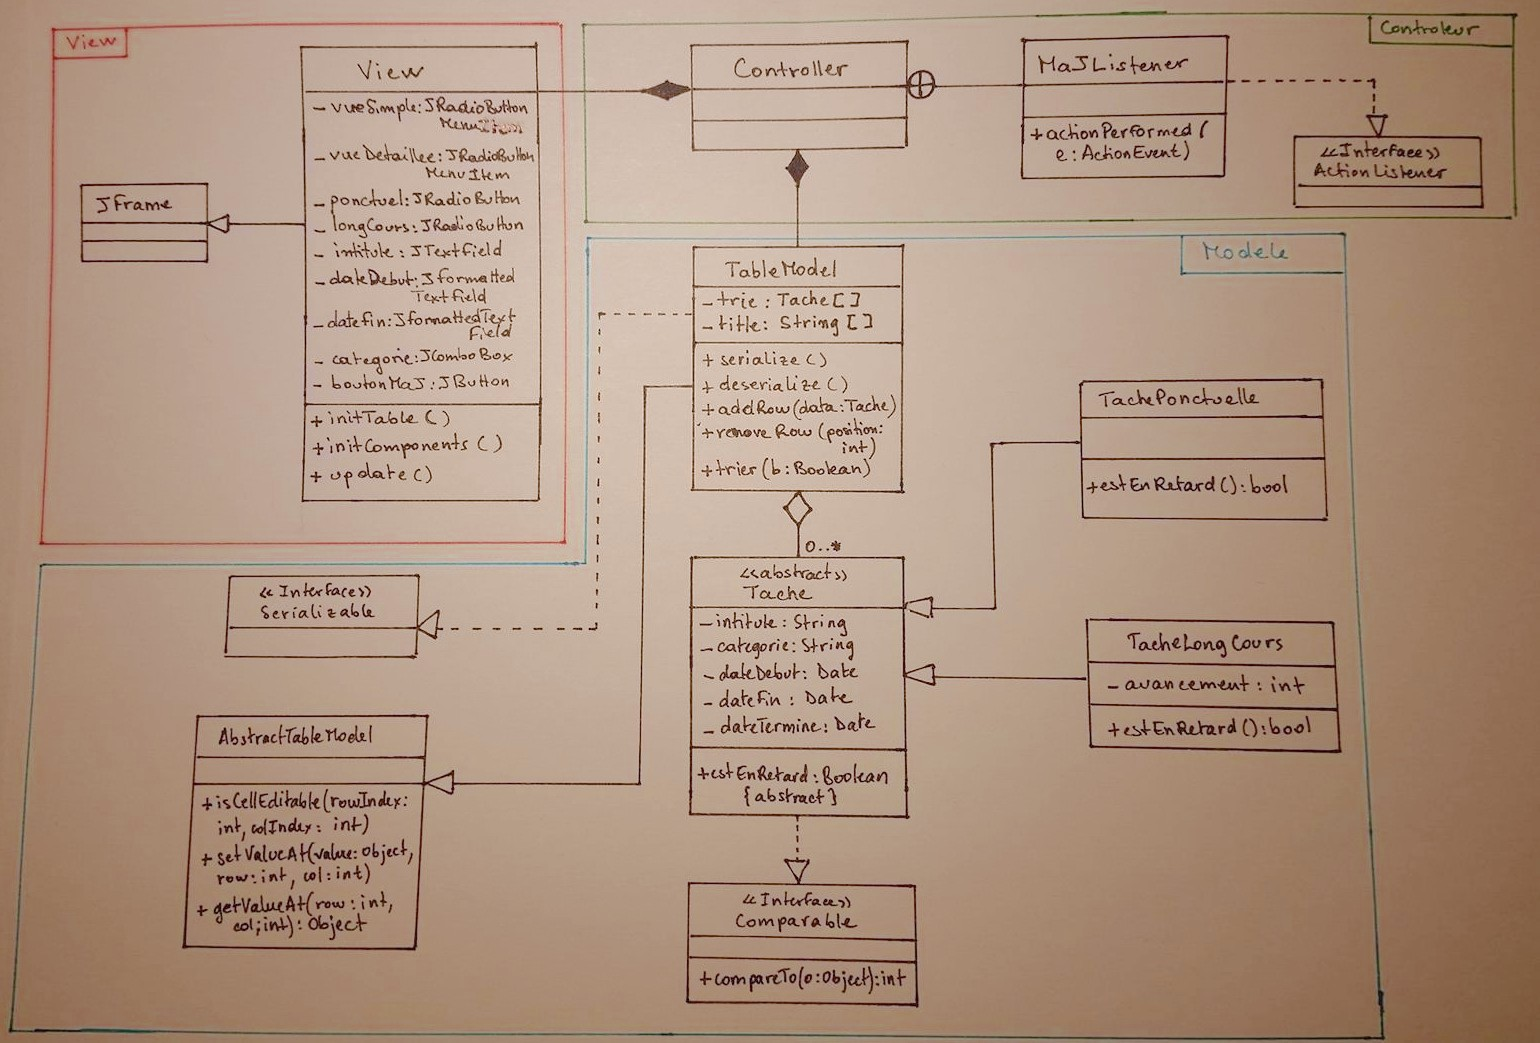
\includegraphics[scale=0.30]{class.jpg}
\caption{Diagramme de Classes}\label{DiagClass}
\end{figure}

\begin{figure}
\centering
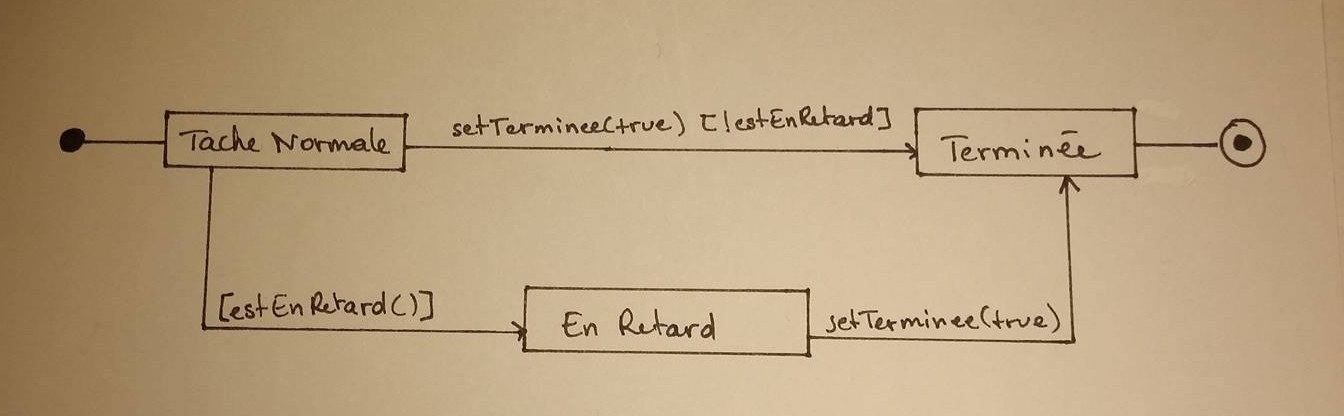
\includegraphics[scale=0.30]{etat.jpg}
\caption{Diagramme d'état-transitions de la classe Tache}\label{etat}
\end{figure}

\begin{figure}
\centering
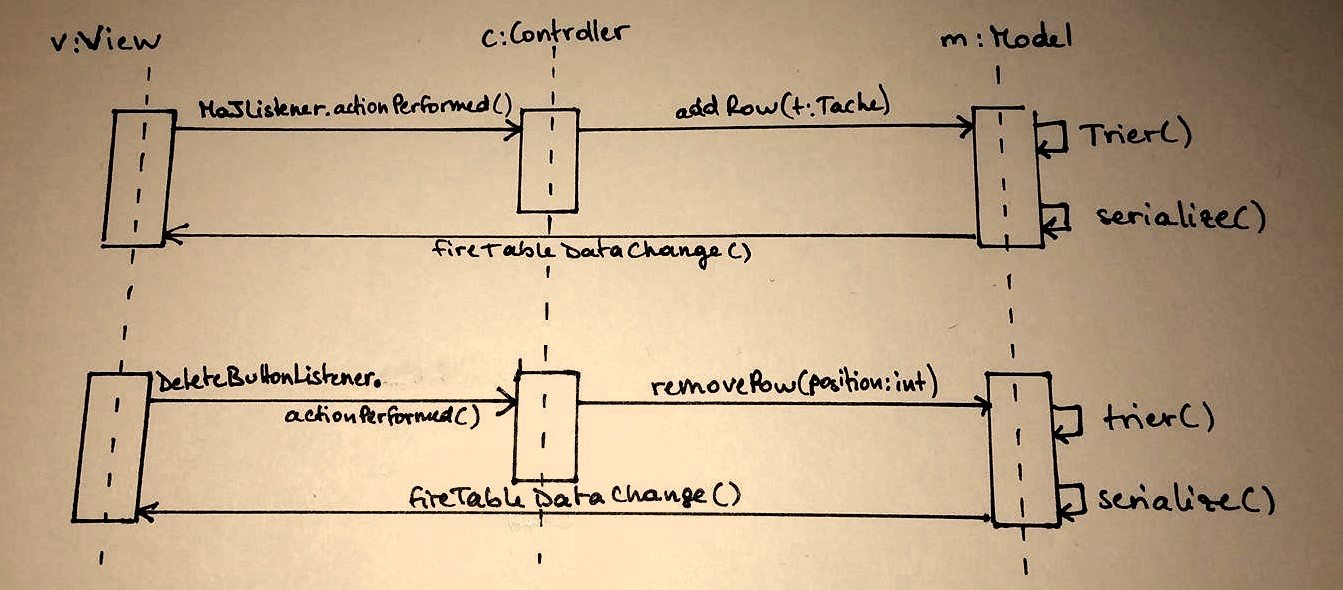
\includegraphics[scale=0.30]{seq.jpg}
\caption{Diagramme de séquence de notre architecture MVC}\label{seq}
\end{figure}

\newpage
\section{Réalisation}
Au vu de notre manque de bases solides sur le MVC, nous avons cherché des tutoriels sur ce sujet. Beaucoup utilisaient le Patern Observer, avec la vue qui contient le controleur, qui contient le modèle, mais cette façon de faire ne nous convenait pas, compte tenu du sujet. Nous avons donc décidé de nous baser sur le tutoriel video de Derek Banas (un anglophone qui a réalisé un série de tutoriels sur les patrons de conception en java). 

Le lien de la video : https://www.youtube.com/watch?v=dTVVa2gfht8

Au final, le controleur contient le modèle et la vue en données membre, et l'interaction entre ceux ci parait plus évidente et claire.

\section{Conclusion}
Pour conclure, nous avons décidé de plus mettre notre temps à profit sur la phase de conception et d'analyse. La phase de réalisation s'est avérée assez productive pour la semaine et demi que nous lui avons allouée. 

\end{document}
